\documentclass[../main.tex]{subfiles}

\begin{document}

\section{Elementos sometidos a tracción axil}

En principio, para este tipo de problemas, primero debemos considerar el área
que estará siendo traccionada. Podemos distinguir tres tipos:

\begin{itemize}
  \item \textbf{Área bruta}. $A_g$
  \item  \textbf{Área neta} $A_n$ : es el área descontando los agujeros para 
    bulones. En caso de estar en tresbolillo, se debe considerar una formula
    especial.
  \item \textbf{Área neta efectiva} $A_e$ : es el área neta teniendo en cuenta el
    \textit{retraso de cortante}, que se da cuando no todos los elementos estan
    conectados directamente. Ver \Cref{retraso-cortante}
\end{itemize}

El $A_e$ puede obtenerse con la formula $A_e = A_n * U$ donde U sale de:

\begin{align*}
  U = 1 - (\overline{x}/L)\leq 0.9
.\end{align*}

Donde el valor de $\overline{x}$ será la excentricidad de la unión, es decir la 
distancia entre el baricentro del agujero hasta el baricentro de la pieza. En
caso de una pieza con dos alas donde se cuenta con una sola línea de bulones,
se considera unicamente los elementos directamente unidos.

\subsection{Retraso de cortante}

Se da cuando tenemos uniones donde no todos los elementos solicitados estan
conectados directamente. Esto se puede ver en \Cref{fig:retraso-cortante}. Vemos 
que no hay fomra física que la parte última de la pieza no conectada trasmita
tensiones.

\begin{figure}[htpb]
  \centering
  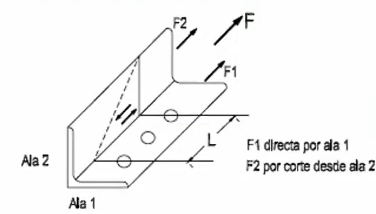
\includegraphics[width=0.8\textwidth]{../images/20210412/retrasocortante}
  \caption{Esquema de retraso de cortante}
  \label{fig:retraso-cortante}
\end{figure}


\end{document}

